
\begin{abstract}
Originating in ergodic structure theory, nilspace theory is concerned with the study of cubical spaces.
A first key result in this theory, the \emph{weak structure theorem}, is the representation of a concrete fibrant compact cubespace as
a tower of its canonical truncations, exhibiting each step over the previous one as a principal bundle by a compact abelian group.
We present a categorical proof of the weak structure theorem by systematically interpreting the relevant concepts in an appropriate context.


\end{abstract}

\tableofcontents
\clearpage

\section{Introduction}

The theory of \emph{nilspaces} originally emerged in the late 2010s after Host and Kra and independently Ziegler proved the convergence of multiple ergodic averages \cite{Host2005,Ziegler2006} by means of what is now called \emph{Host-Kra structure theory} \cite{Host2018,Eisner2025}.
One of the key insights in their proofs is that every ergodic measure-preserving $\Z$-system $X$
decomposes into \emph{structured factors $Z_k$} which capture the convergence behavior of the $k+1$-fold ergodic averages (or: the factors are \emph{characteristic} for the convergence of the $k$-fold ergodic averages),
and \emph{random parts $Z_k^\perp$} on which the $k+1$-fold ergodic averages tend to zero.
The first two such decompositions are easy to describe:
$Z_0$ is the invariant factor of the system, i.e., where the action is trivial,
and corresponds to von Neumann's Mean Ergodic Theorem,
and $Z_1$ is the \emph{Kronecker factor} on which the system is a rotational system on a compact abelian group by the Halmos-von Neumann Theorem.
The $Z_k$ make up a tower of factors of $X$
\begin{center}
\begin{tikzcd}[ampersand replacement=\&]
	X \& \dots \& {Z_{k}} \& {Z_{k-1}} \& \dots \& {Z_1} \& {Z_0}
	\arrow[two heads, from=1-1, to=1-2]
	\arrow[two heads, from=1-2, to=1-3]
	\arrow[two heads, from=1-3, to=1-4]
	\arrow[two heads, from=1-4, to=1-5]
	\arrow[two heads, from=1-5, to=1-6]
	\arrow[two heads, from=1-6, to=1-7]
\end{tikzcd}
\end{center}
which exhibits $Z_k$ as a skew-product extension of $Z_{k-1}$ by a compact abelian group $A_k$,
i.e., this tower is an iterated abelian bundle.
This statement is known under the name of \emph{weak structure theorem}.
From there, the \emph{strong structure theorem} describes the system $Z_k$ as a limit of translational systems on $k$-step nilmanifolds,
i.e., translational systems on a homogeneous space $G/\Lambda$ where $G$ is a $k$-step nilpotent Lie group and $\Lambda$ is a lattice therein.
This description is sufficient to prove convergence of the $k$-fold ergodic averages,
see also \cite{Leibman2006}.

Interestingly, underlying the Host-Kra theory there are many \emph{cubical patterns} \cite{Host2004,Host2005,Host2005a,Host2008, Host2010}.
In fact, the Host-Kra factors are the universal characteristic factors for cubical ergodic averages,
and Host-Kra-Gowers semi-norms, cubegroups and iterated self-joinings
are described using indices describing the combinatorial behavior of discrete cubes ${\bbox}^n = \{0,1\}^n$.
Extracting the algebraic properties of these cubical patterns is at the core of nilspace theory,
pioneered by Antol\'in Camarena and Szegedy in \cite{Camarena2010},
who exploit the cubical patterns to obtain an analogous weak and strong structure theorem,
showing that what matters is not the ergodic system itself
but merely its underlying cubical structure.
More groundwork on nilspaces has been put forward in a series of papers by Gutman, Manners and Varj\'u \cite{Gutman2020,Gutman2020a,Gutman2020b}
and by Candela \cite{Candela2017,Candela2017a},
who both systematized and improved the weak and strong structure theorem for nilspaces.
From there, it is straightforward to deduce topological Host-Kra theory \cite{Host2010,Shao2012}
from the strong structure theory of nilspaces, see \cite{Glasner2018,Gutman2020b,Glasner2023}.
But nilspace theory also gives ways of proving the strong structure theorem for measure-preserving systems,
as in \cite{Gutman2023} and \cite{Candela2020,Candela2023}.
Apart from its applications to ergodic theory, nilspace theory has many other applications,
e.g. in Inverse Gowers Theory, Higher Order Fourier Analysis and additive combinatorics,
see \cite{Candela2021,Candela2022,Jamneshan2026d}.

\subsection*{Overview}

The goal of this text is to give a new proof of (a generalized version of) the following theorem.

\begin{theorem*}[Corollary~\ref{cor:compact-weak-structure}]
Let $X$ be a compact ergodic nilspace.
Then there is a tower of surjective fibrations
\begin{center}
\begin{tikzcd}
	X & \cdots & {\tau_2X} & {\tau_1X} & {\tau_0X}
	\arrow[from=1-1, to=1-2]
	\arrow[from=1-2, to=1-3]
	\arrow[from=1-3, to=1-4]
	\arrow[from=1-4, to=1-5]
\end{tikzcd}
\end{center}
such that $\tau_n X$ is a compact $n$-step nilspace
and the compact group $\pi_n(X,x_0)$ acts freely on $\tau_n X$
such that the orbits are the fibers of the quotient $\tau_n X\to\tau_{n-1} X$.
\end{theorem*}

To do so, we thoroughly study and introduce the concepts of cubesets, fibrations, truncations, structure groups and related notions
from a categorical point of view.

The central definition in nilspace theory is that of a \emph{cubeset} $X$.
It consists of a family of sets $X(n)$ of $n$-dimensional cubes for every $n\in\N$,
compatible with certain restriction maps.
This information can be encoded in that $X$ is a \emph{presheaf} on cubes.
Rather than saying what a single cube is, it is easier to say what the category of cubes is,
i.e., how the cubes of different dimension interact with each other.

\begin{definition*}[Definition~\ref{def:cube_cat}]
The \emph{category of cubes $\bbox$} is the category with objects ${\bbox}^n = \{0,1\}^n$ for $n\in\N_0$
and morphisms $f\colon{\bbox}^n\to{\bbox}^m$ given by affine linear maps $\Z^n\to\Z^m$ that map $\{0,1\}^n$ into $\{0,1\}^m$.
\end{definition*}

The first $n$-cubes can be pictured as follows, drawing the images of every injective map into the cube.

\begin{center}

\pgfdeclarelayer{symfacefill}
\pgfdeclarelayer{symfaceoutline}
\pgfsetlayers{symfacefill,symfaceoutline,main}


\newcommand{\SymFace}[1]{%
  \begin{pgfonlayer}{symfacefill}
    \path[fill=gray, fill opacity=0.10] #1 -- cycle;
  \end{pgfonlayer}
  \begin{pgfonlayer}{symfaceoutline}
    \path[draw=gray!60,line width=0.45pt] #1 -- cycle;
  \end{pgfonlayer}
}


\newcommand{\SymDiagFace}[1]{%
  \begin{pgfonlayer}{symfacefill}
    \path[fill=gray, fill opacity=0.16] #1 -- cycle;
  \end{pgfonlayer}
  \begin{pgfonlayer}{symfaceoutline}
    \path[draw=gray!70,line width=0.5pt] #1 -- cycle;
  \end{pgfonlayer}
}


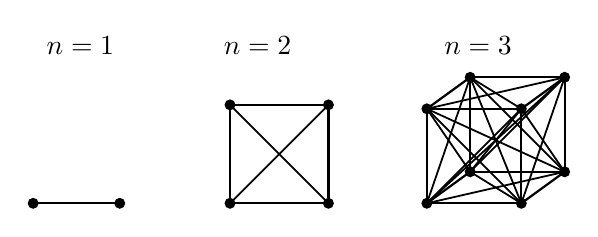
\begin{tikzpicture}[
    x=1cm,y=1cm,
    font=\small,
    line cap=round,
    line join=round,
    vertex/.style={circle,fill,inner sep=1.4pt},
    mainedge/.style={draw=black, line width=0.8pt},
    affdiag/.style={draw=black, line width=0.65pt},
    simpedge/.style={
        draw=black,
        line width=0.75pt,
        -{Stealth[length=1.6mm,width=1.1mm]},
        shorten <= 8.0pt,
        shorten >= 8.0pt
    },
    rowlab/.style={anchor=east},
    collab/.style={font=\normalsize},
scale=0.5
]



\node[collab] at ( 1.2,  4.0) {$n=1$};
\node[collab] at ( 5.7,  4.0) {$n=2$};
\node[collab] at (11.3,  4.0) {$n=3$};

\begin{scope}
    \coordinate (A) at (0,0);
    \coordinate (B) at (2.2,0);


    \draw[mainedge] (A)--(B);
    \node[vertex] at (A) {};
    \node[vertex] at (B) {};
\end{scope}


\begin{scope}[shift={(5,0)}]
    \coordinate (A) at (0,0);
    \coordinate (B) at (2.5,0);
    \coordinate (C) at (0,2.5);
    \coordinate (D) at (2.5,2.5);


    \SymFace{(A)--(B)--(D)--(C)}


    \draw[mainedge] (A)--(B);
    \draw[mainedge] (B)--(D);
    \draw[mainedge] (D)--(C);
    \draw[mainedge] (C)--(A);


    \draw[affdiag] (A)--(D);
    \draw[affdiag] (B)--(C);


    \foreach \P in {A,B,C,D} {
        \node[vertex] at (\P) {};
    }
\end{scope}


\begin{scope}[shift={(10,0)}]
    \coordinate (A) at (0,0);
    \coordinate (B) at (2.4,0);
    \coordinate (C) at (0,2.4);
    \coordinate (D) at (2.4,2.4);


    \coordinate (E) at (1.1,0.8);
    \coordinate (F) at (3.5,0.8);
    \coordinate (G) at (1.1,3.2);
    \coordinate (H) at (3.5,3.2);


    \SymFace{(A)--(B)--(D)--(C)}
    \SymFace{(E)--(F)--(H)--(G)}
    \SymFace{(A)--(B)--(F)--(E)}
    \SymFace{(C)--(D)--(H)--(G)}
    \SymFace{(A)--(C)--(G)--(E)}
    \SymFace{(B)--(D)--(H)--(F)}


    \SymDiagFace{(A)--(B)--(H)--(G)}
    \SymDiagFace{(A)--(C)--(H)--(F)}
    \SymDiagFace{(A)--(E)--(H)--(D)}


    \draw[mainedge] (A)--(B);
    \draw[mainedge] (B)--(D);
    \draw[mainedge] (D)--(C);
    \draw[mainedge] (C)--(A);


    \draw[mainedge] (E)--(F);
    \draw[mainedge] (F)--(H);
    \draw[mainedge] (H)--(G);
    \draw[mainedge] (G)--(E);


    \draw[mainedge] (A)--(E);
    \draw[mainedge] (B)--(F);
    \draw[mainedge] (C)--(G);
    \draw[mainedge] (D)--(H);


    \draw[affdiag] (A)--(D);
    \draw[affdiag] (B)--(C);
    \draw[affdiag] (E)--(H);
    \draw[affdiag] (F)--(G);
    \draw[affdiag] (A)--(F);
    \draw[affdiag] (B)--(E);
    \draw[affdiag] (C)--(H);
    \draw[affdiag] (D)--(G);
    \draw[affdiag] (A)--(G);
    \draw[affdiag] (C)--(E);
    \draw[affdiag] (B)--(H);
    \draw[affdiag] (D)--(F);


    \draw[affdiag] (A)--(H);
    \draw[affdiag] (B)--(G);
    \draw[affdiag] (C)--(F);
    \draw[affdiag] (D)--(E);


    \foreach \P in {A,B,C,D,E,F,G,H} {
        \node[vertex] at (\P) {};
    }
\end{scope}
\end{tikzpicture}
\end{center}

There is an important subclass of morphisms in $\bbox$:
the morphisms $f\colon{\bbox}^n\to{\bbox}^m$ that are the restriction of a linear map.
Since they also have to map the unit cube $\{0,1\}^n$ into the unit cube,
each such linear map arises from a (not necessarily invertible) permutation of coordinates and thus
is characterized by a map of sets $\{1,\ldots,m\}\to\{1,\ldots,n\}$.
There's only one caveat: it might be possible for $f$ to be constant zero in some coordinates,
so the map of sets $\{1,\ldots,m\}\to\{1,\ldots,n\}$ only is partially defined.

\begin{definition*}[Definition~\ref{def:indexcats}]
\emph{Segal's category $\bbGamma$} is the opposite of the category of finite sets
and partially defined maps.
\end{definition*}

With this adapted category, every morphism indeed arises as a coordinate permutation
which upgrades to an equivalence of categories.

\begin{proposition*}[Proposition~\ref{lem:iso-gamma-bblox}]
There is an equivalence of categories between $\bbGamma$ and the subcategory of $\bbox$
consisting of the linear maps.
\end{proposition*}

It turns out that there is a purely categorical, coordinate-free construction to arrive from Segal's category $\bbGamma$
at the category of cubes $\bbox$.

\begin{proposition*}[Proposition~\ref{prop:cube_cat_linear}]
The cube category $\bbox$ is the unstraightening
\[
    \mathrm{Un}(\ast/\F_2^\bullet)=\int_{\bbGamma} \ast/\F_2^\bullet\to\bbGamma
\]
of the functor $\ast/\F_2^\bullet\colon\bbGamma\to\Cat$ that assigns to every $n$-element set
the delooping of the group $\F_2^n = (\Z/2\Z)^n$.
\end{proposition*}

This proposition ultimately relies on the fact that a morphism of cubes
can be uniquely decomposed into a linear map followed by a \emph{flip},
i.e. a map that only reverses the orientation of the cube along certain coordinate axes
(Lemma~\ref{lem:linearization-auto-bblox}).
The description of the cube category $\bbox$ as unstraightening over $\bbGamma$
now enables us to lift certain nice properties of $\bbGamma$ to $\bbox$:
among them a classification of epi- and monomorphisms (Lemma~\ref{lem:bbox-epi-mono}),
the existence of a Cisinski generalized Reedy structure (Lemma~\ref{lem:bbox-reedy-cat})
and the cartesian monoidal structure (Corollary~\ref{prop:bbox-symm-monoid}).

Now given the basic building blocks for the theory, a \emph{cubeset $X$} is some kind of space made out of cubes.
So $X$ consists of a collection of $n$-cubes $X(n)$ for every $n\in\N_0$,
and for any map $f\colon{\bbox}^n\to{\bbox}^m$ between cubes,
there is a restriction $X(f)\colon X(m)\to X(n)$, compatible with composition and the identity map.
This justifies calling the set $X(n)$ the collection of $n$-cubes.

\begin{definition*}[Definition~\ref{def:cubeset}]
A \emph{cubeset $X$} is a presheaf of sets on the category of cubes $\bbox$,
and the category $\cSet$ of cubesets is the presheaf category $\PSh(\bbox)=\Fun(\bbox^\op,\Set)$.
\end{definition*}

We briefly recall all relevant properties of the presheaf category of cubes in Section~\ref{ssec:cubesets-basics} and study their relation to presheaves on $\bbGamma$.
Most notably, we give an alternative description of the presheaf category
over a category that arises as the Grothendieck construction of a functor $F\colon\cC\to\Grp$
(Proposition~\ref{prop:unstrait-presehaf}).
The three main examples of cubesets are also given in this section:

\begin{example*}[Lemma~\ref{lem:point-cset}]
Given a set $S$, the \emph{trivial cubeset $i_!S$} is given by the constant presheaf
that assigns to an $n$-cube ${\bbox}^n$ the set $S$ and to a map of cubes the identity on $S$.

The \emph{discrete cubeset $i_\ast S$} is given by the presheaf
\[
    {\bbox}^n\mapsto\hom_{\set}(\{0,1\}^n,S).
\]
\end{example*}

\begin{example*}[Example~\ref{ex:host_kra_cubegroups}]
Given an abelian group $A$ and $k\in\N$ we define the \emph{$k$-th Eilenberg-Mac Lane cubeset $\cD_k(A)$} to be the subcubeset of $i_\ast A$ whose $n$-cubes are the subgroup of $A^{2^n}$ generated by elements of the form
\[
    a^F\colon\{0,1\}^n\to A,\quad\omega\mapsto\begin{cases}
        a,\quad & \omega\in F, \\
        0,\quad & \omega\notin F,
    \end{cases}
\]
where $F$ runs over all cube faces of $\{0,1\}^n$
whose dimension is at least $n-k$ and $a$ is an element of $A$.
\end{example*}

In practice, the relevant cubesets, and in particular, all examples considered above,
have the additional property of \emph{concreteness}.
A cubeset $X$ is concrete if each $n$-cube of $X$ is fully determined by its vertices.

\begin{definition*}[Definition~\ref{def:concrete-cubeset}]
A cubeset $X$ is \emph{concrete} if the natural map
\[
    X(n) \to \prod_{0\to n} X(0) = X(0)^{2^n}
\]
is injective.
We denote the full subcategory of concrete cubesets by $\ccSet$.
\end{definition*}

Since concreteness is defined via limits, concrete cubesets are stable under limits
and thus there is a \emph{concretification}, i.e. a left adjoint to the inclusion,
that assigns to a cubeset $X$ an associated concrete cubeset (Proposition~\ref{prop:concrete-left-adjoint}).
The rest of Section~\ref{ssec:concrete-cubesets} deals with stability properties of
concrete cubesets: they are stable under coproducts, filtered colimits, internal Hom and subobjects.

Another important aspect of cubesets is \emph{corner completion}.

\begin{definition*}[Definition~\ref{def:corner}]
For $n\in\N$, the \emph{$n$-corner ${\bbcor}^n$} is the union of all linear faces of ${\bbox}^n$
of dimension less than $n$ that don't contain the point $1^n=(1,\ldots,1)$.
\end{definition*}

The first few $n$-corners look as follows.
\begin{center}

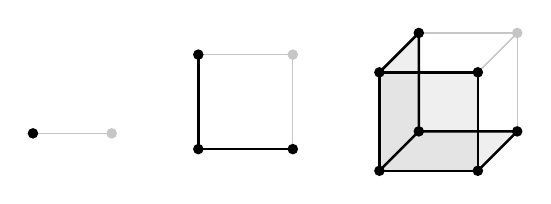
\begin{tikzpicture}[
    x=1cm,y=1cm,
    font=\small,
    line cap=round,
    line join=round,
    vertex/.style={circle,fill,inner sep=1.35pt},
    greyvertex/.style={circle,fill=gray!45,inner sep=1.35pt},
    ambient/.style={draw=gray!45,line width=0.45pt},
    corneredge/.style={draw=black,line width=0.9pt},
    cornerface/.style={
        draw=gray!55,
        fill=gray!45,
        line width=0.45pt,
        fill opacity=0.28
    },
    toplabel/.style={font=\normalsize},
scale=0.5
]

\begin{scope}[shift={(0,0)}]
    \coordinate (A) at (0,0);
    \coordinate (B) at (2,0);

    \draw[ambient] (A)--(B);

    \node[vertex] at (A) {};
    \node[greyvertex] at (B) {};
\end{scope}

\begin{scope}[shift={(4.2,-0.4)}]
    \coordinate (A) at (0,0);
    \coordinate (B) at (2.4,0);
    \coordinate (C) at (0,2.4);
    \coordinate (D) at (2.4,2.4);

    \draw[ambient] (A)--(B)--(D)--(C)--cycle;

    \draw[corneredge] (A)--(B);
    \draw[corneredge] (A)--(C);

    \node[vertex] at (A) {};
    \node[vertex] at (B) {};
    \node[vertex] at (C) {};
    \node[greyvertex] at (D) {};
\end{scope}


\begin{scope}[shift={(8.8,-0.95)}]
    \coordinate (A) at (0,0);
    \coordinate (B) at (2.5,0);
    \coordinate (C) at (0,2.5);
    \coordinate (D) at (2.5,2.5);

    \coordinate (E) at (1.0,1.0);
    \coordinate (F) at (3.5,1.0);
    \coordinate (G) at (1.0,3.5);
    \coordinate (H) at (3.5,3.5);

    \draw[ambient] (A)--(B)--(D)--(C)--cycle;
    \draw[ambient] (E)--(F)--(H)--(G)--cycle;
    \draw[ambient] (A)--(E);
    \draw[ambient] (B)--(F);
    \draw[ambient] (C)--(G);
    \draw[ambient] (D)--(H);

    \filldraw[cornerface] (A)--(B)--(D)--(C)--cycle;
    \filldraw[cornerface] (A)--(B)--(F)--(E)--cycle;
    \filldraw[cornerface] (A)--(C)--(G)--(E)--cycle;

    \draw[corneredge] (A)--(B)--(D)--(C)--cycle;
    \draw[corneredge] (A)--(E)--(F)--(B);
    \draw[corneredge] (E)--(G)--(C);

    \draw[ambient] (D)--(H);
    \draw[ambient] (F)--(H);
    \draw[ambient] (G)--(H);

    \foreach \P in {A,B,C,D,E,F,G}
        \node[vertex] at (\P) {};

    \node[greyvertex] at (H) {};
\end{scope}

\end{tikzpicture}
\end{center}

This leads to the definition of a fibrant cubeset and the relative version thereof, a \emph{fibration}.

\begin{definition*}[Definition~\ref{def:nil-fibration}]
    \begin{enumerate}[(i)]
        \item
A cubeset $X$ is called \emph{fibrant} if it has \emph{corner completion},
i.e., for every corner ${\bbcor}^n\to X$ in $X$ there exists a completion to a cube ${\bbox}^n\to X$
along the inclusion ${\bbcor}^n\to{\bbox}^n$.

        \item
A map $f\colon X\to Y$ between cubesets is called \emph{fibration},
if for every commutative diagram
\begin{center}
\begin{tikzcd}[ampersand replacement=\&]
	{{\bbcor}^n} \& X \\
	{{\bbox}^n} \& Y
	\arrow[from=1-1, to=1-2]
	\arrow[hook, from=1-1, to=2-1]
	\arrow[from=1-2, to=2-2]
	\arrow[dashed, from=2-1, to=1-2]
	\arrow[from=2-1, to=2-2]
\end{tikzcd}
\end{center}
there exists a diagonal lift ${\bbox}^n\to X$.
        \end{enumerate}
\end{definition*}

This means that every $n$-corner in $X$ that can be completed in $Y$ to an $n$-cube already has a completion to an $n$-cube in $X$ which maps to the cube in $Y$.

The notion of fibration originates in model categories and is usually defined
via a right lifting property against a set of morphisms,
as is the case for fibrations of cubesets.
Applying Quillen's small object argument, we obtain a weak factorization system:
two classes of morphisms $(l(r(\Lambda)),r(\Lambda))$ such that each map of cubesets
decomposes into
\begin{center}
\begin{tikzcd}
	X & W & Y
	\arrow["h", tail, from=1-1, to=1-2]
	\arrow["f"', curve={height=12pt}, from=1-1, to=1-3]
	\arrow["g", two heads, from=1-2, to=1-3]
\end{tikzcd}
\end{center}
where $g$ is a fibration and $h$ is a \emph{trivial cofibration},
meaning that it belongs to the class $l(r(\Lambda))$, see Section~\ref{ssec:fibrations}.
There is also an explicit construction of trivial cofibrations
starting from corner inclusions ${\bbcor}^n\to{\bbox}^n$ (Construction~\ref{cons:triv-cofib}).
This gives a generalization of the extension property of simplicial cubesets from \cite[Lemma 3.1.5]{Candela2017} and \cite[Lemma 7.5]{Gutman2020}.

\begin{proposition*}[Proposition~\ref{prop:triv-nilcofib-simp}]
Let $K$ be a non-empty downwards-closed collection of subsets of $\{1,\ldots,n\}$.
Then the inclusion
\[
    \bigcup_{A\in K}{\bbox}^{\lvert A\rvert}\to{\bbox}^n
\]
is a trivial cofibration.
\end{proposition*}

The rest of the section on fibrations deals with fibrant replacements
and their interaction with concrete cubesets,
as well as with stability properties of fibrations and trivial cofibrations.

Following this theme we introduce cubesets with gluing property.
Informally, a cubeset $X$ has the gluing property if, for any two $n$-cubes $a$ and $b$ in $X$
that share a common face of dimension $n-1$,
we can glue them along this face to a new cube $c$ of $X$.
To make this precise, we define a class of morphisms $\bprism$,
and then define the gluing property to be a right lifting property against the morphisms in $\bprism$
(Definition~\ref{def:gluing-property}).
It turns out that a cubeset $X$ with the gluing property, such that the gluing of any two cubes is unique, already is concrete (Proposition~\ref{prop:unique-gluing-concrete}).
Moreover, each fibrant cubeset has the gluing property (Proposition~\ref{prop:nilfib-gluing}).

In Section~\ref{ssec:corner-gamma} we give an alternative description of corner completion.
Every cubeset $X$ can be interpreted as a $\bbGamma$-set $j^\ast X$
whose $n$-cubes are just the $n$-cubes of $X$, but we only consider maps $X(m)\to X(n)$
that arise from linear maps of cubes (Remark~\ref{rem:adjoint-triple-j}).

\begin{definition*}[Definition~\ref{def:omega_corner_gamma}]
Let $n\in\N$ and $\omega\in\{0,1\}^n\setminus\{0^n\}$.
Then define the $n$-corner ${\bbcor}^n_\omega$ w.r.t. $\omega$ as the union over all injections $f\colon{\bblox}^{n-1}\to{\bblox}^n$ in $\bbGamma$
such that $f$ misses $\omega$, i.e., $\omega\notin\im f$:
\[
    {\bbcor}^n_\omega = \bigcup_{\substack{f\colon{\bblox}^{n-1}\sub{\bblox}^n \\ \omega\notin\im f}}{\bblox}^{n-1}\hookrightarrow{\bblox}^n.
\]
\end{definition*}

In two dimensions, those corners look as follows.
\begin{center}
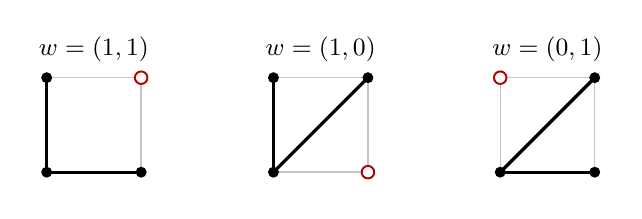
\begin{tikzpicture}[
    scale=0.6,
    line cap=round,
    line join=round,
    bg/.style={draw=gray!45, line width=0.5pt},
    face/.style={draw=black, line width=1.2pt},
    vtx/.style={circle, fill=black, inner sep=1.4pt},
    missing/.style={circle, draw=red!70!black, fill=white, line width=0.7pt, inner sep=1.6pt},
    lab/.style={font=\scriptsize},
    title/.style={font=\small\bfseries}
]


\begin{scope}[shift={(0,0)}]
  \node[title] at (1,2.6) {$w=(1,1)$};

  \coordinate (O) at (0,0);
  \coordinate (A) at (2,0);
  \coordinate (B) at (0,2);
  \coordinate (C) at (2,2);

  \draw[bg] (O)--(A)--(C)--(B)--cycle;

  \draw[face] (O)--(A);
  \draw[face] (O)--(B);

  \node[vtx] at (O) {};
  \node[vtx] at (A) {};
  \node[vtx] at (B) {};
  \node[missing] at (C) {};

  \node[lab, below left]  at (O) {};
  \node[lab, below right] at (A) {};
  \node[lab, above left]  at (B) {};
  \node[lab, above right] at (C) {};
\end{scope}


\begin{scope}[shift={(4.8,0)}]
  \node[title] at (1,2.6) {$w=(1,0)$};

  \coordinate (O) at (0,0);
  \coordinate (A) at (2,0);
  \coordinate (B) at (0,2);
  \coordinate (C) at (2,2);

  \draw[bg] (O)--(A)--(C)--(B)--cycle;

  \draw[face] (O)--(B);
  \draw[face] (O)--(C);

  \node[vtx] at (O) {};
  \node[missing] at (A) {};
  \node[vtx] at (B) {};
  \node[vtx] at (C) {};

  \node[lab, below left]  at (O) {};
  \node[lab, below right] at (A) {};
  \node[lab, above left]  at (B) {};
  \node[lab, above right] at (C) {};
\end{scope}


\begin{scope}[shift={(9.6,0)}]
  \node[title] at (1,2.6) {$w=(0,1)$};

  \coordinate (O) at (0,0);
  \coordinate (A) at (2,0);
  \coordinate (B) at (0,2);
  \coordinate (C) at (2,2);

  \draw[bg] (O)--(A)--(C)--(B)--cycle;

  \draw[face] (O)--(A);
  \draw[face] (O)--(C);

  \node[vtx] at (O) {};
  \node[vtx] at (A) {};
  \node[missing] at (B) {};
  \node[vtx] at (C) {};

  \node[lab, below left]  at (O) {};
  \node[lab, below right] at (A) {};
  \node[lab, above left]  at (B) {};
  \node[lab, above right] at (C) {};
\end{scope}

\end{tikzpicture}
\end{center}

Now for a general cubeset, there is no reason as to why fibrancy against the (classical) corner in $\bbox$ implies fibrancy against the corner ${\bbcor}^n_\omega$ in $\bbGamma$.
However, if $X$ is concrete, then one cannot distinguish between those notions.

\begin{proposition*}[Proposition~\ref{prop:nilfib-restricted-nilfib-concrete}]
Let $X$ be a concrete cubeset.
Then the following assertions are equivalent.
\begin{enumerate}[(a)]
    \item The cubeset $X$ is fibrant.
    \item The underlying $\bbGamma$-set of $X$ is fibrant w.r.t. the corner inclusions
            ${\bbcor}^n_\omega\to{\bblox}^n$.
\end{enumerate}
\end{proposition*}

Another important property of a cubeset is its \emph{step}.

\begin{definition*}[Definition~\ref{def:n-step}]
A cubeset $X$ is called \emph{$k$-step} if for all $n\geq k+1$ the map
\[
    \hom({\bbox}^n, X) \to \hom({\bbcor}^n, X)
\]
is bijective, i.e., each $n$-corner in $X$ has a unique completion to an $n$-cube of $X$.
The full subcategory of $k$-step cubesets is denoted $\cSet_k$.
\end{definition*}

This means that if $X$ is $k$-step, its collection of $n$-cubes for $n>k$ is fully determined
by the $k$-cubes of $X$.
We give multiple equivalent characterizations of $k$-step cubesets in Proposition~\ref{prop:truncations-char}.
Given a general cubeset $X$, one can associate to it the maximal $k$-step quotient $\tau_k X$,
meaning that every other map $X\to Y$ where $Y$ is $k$-step factors through $X\to \tau_k X$.
Speaking categorically this states that the inclusion $\cSet_k\to\cSet$ admits a left adjoint
$\tau_k\colon\cSet\to\cSet_k$ (Proposition~\ref{prop:step-left-adjoint}).
This left adjoint preserves finite products (Proposition~\ref{prop:n-trunc-ihom-prod})
and we give stability conditions on $k$-step cubesets in Proposition~\ref{prop:n-trunc-closure}.
In general, it is not easy to compute the $k$-step quotient $\tau_k X$ of $X$.
However, if $X$ is concrete and fibrant, then a process called \emph{universal replacement}
yields $\tau_k X$ as an easy-to-compute factor of $X$.

\begin{definition*}[Definition~\ref{def:univ-replacement}]
For $x,y\in X(0)$ define $x\sim_k y$ if there exist ($k+1$)-cubes in $X$ that agree on the corner and have $x$ and $y$ on their uppermost vertex $1^{k+1}$, respectively.
\end{definition*}

This equivalence relation on $X(0)$ induces a factor $X(0)/\sim_k$
which yields a new cubeset $X/\sim_k$ whose $n$-cubes $X/\sim_k(n)$ are given by the image of $X(n)$ under the projection
\[
    X(0)^{2^n}\to (X(0)/\sim_k)^{2^n}.
\]
Explicitly this means that two $n$-cubes in $X$ are identified if all their points are equivalent in $X(0)$.

\begin{proposition*}[Proposition~\ref{prop:trunc_concfib}]
Let $X$ be a concrete fibrant cubeset.
Then the truncation $\tau_k X$ is given by $X/\sim_k$.
Moreover, the unit $\eta\colon X\to\tau_k X$ is a surjective fibration
and $\tau_k X$ is concrete and fibrant.
\end{proposition*}

This proposition generalizes the well-known fact that $\sim_k$ is the smallest equivalence relation
on $X(0)$ such that $X/\sim_k$ is $k$-step, see \cite[Proposition 6.3]{Gutman2020}.

In Section~\ref{ssec:connectivity} we further investigate the $0$-truncation of a (general) cubeset.
This includes the definition of \emph{ergodicity}.

\begin{definition*}[Definition~\ref{def:ergodic}]
A cubeset $X$ is \emph{$n$-ergodic} if $\tau_{n-1}X = \ast$.
\end{definition*}

We will then describe a decomposition into ergodic components (Proposition~\ref{prop:ergodic-decomp}).
Also, there is the analogous concept for $\bbGamma$-sets.
In Section~\ref{ssec:truncation-gamma} we compute the truncation over $\bbGamma$
for concrete cubesets which continues the theme of Section~\ref{ssec:corner-gamma}.

Next, in Section~\ref{ssec:structure-group} we study algebraic invariants of cubesets:
their structure groups.

\begin{definition*}[Definition~\ref{def:structure-group}]
If $X$ is a fibrant cubeset, then an $n$-sphere of $X$ based at $x_0\in X$
is an $n$-cube $s\colon{\bbox}^n\to X$ whose restriction to the $n$-corner is constant $x_0$.
\end{definition*}

Now one would like to use corner completion one dimension higher to define the multiplication of $n$-spheres.
In case $n = 2$, for example, given spheres $c,d$ in $X$
one can build a 3-corner of $X$ which has $c$ on one side, $d$ on another,
and the constant cube $x_0$ on the remaining inert faces.
\begin{center}
\begin{tikzcd}[row sep=small, column sep=small]
	& d &&&& d && {c*d} \\
	{x_0} && c && {x_0} && c \\
	& {x_0} && {x_0} && {x_0} && {x_0} \\
	{x_0} && {x_0} && {x_0} && {x_0}
	\arrow[no head, from=1-6, to=1-8]
	\arrow[dashed, no head, from=1-6, to=3-6]
	\arrow[no head, from=2-1, to=1-2]
	\arrow[no head, from=2-1, to=2-3]
	\arrow[no head, from=2-5, to=1-6]
	\arrow[color={rgb,255:red,214;green,92;blue,92}, no head, from=2-5, to=1-8]
	\arrow[no head, from=2-5, to=2-7]
	\arrow[color={rgb,255:red,214;green,92;blue,92}, no head, from=2-5, to=4-5]
	\arrow[no head, from=2-7, to=1-8]
	\arrow[dashed, no head, from=3-2, to=1-2]
	\arrow[dashed, no head, from=3-2, to=3-4]
	\arrow[dashed, no head, from=3-6, to=3-8]
	\arrow[color={rgb,255:red,214;green,92;blue,92}, no head, from=3-8, to=1-8]
	\arrow[no head, from=4-1, to=2-1]
	\arrow[dashed, no head, from=4-1, to=3-2]
	\arrow[no head, from=4-1, to=4-3]
	\arrow[no head, from=4-3, to=2-3]
	\arrow[no head, from=4-3, to=3-4]
	\arrow[dashed, no head, from=4-5, to=3-6]
	\arrow[color={rgb,255:red,214;green,92;blue,92}, dashed, no head, from=4-5, to=3-8]
	\arrow[no head, from=4-5, to=4-7]
	\arrow[no head, from=4-7, to=2-7]
	\arrow[no head, from=4-7, to=3-8]
\end{tikzcd}
\end{center}
Then using corner completion we obtain the composition $c*d$
by taking the diagonal of the completed 3-cube (depicted in red).
But: composition might not be well-defined.
To account for this deficit, we just define two $n$-spheres to be equivalent if
they both arise as the diagonal of the completion of the same ($n+1$)-corner.
In case that $X$ is a concrete fibrant cubeset, this actually defines an equivalence relation on $n$-spheres,
yielding the set $\pi_n(X,x_0)$ on which we can install the multiplication just described,
see Constructions~\ref{cons:structure-monoid-concrete} and~\ref{cons:concrete-structure-monoid-mult}.

\begin{proposition*}[Propositions~\ref{prop:concrete-structure-group-is-monoid}~and~\ref{prop:concrete-structure-group-is-group}]
Let $X$ be a fibrant concrete cubeset.
The set $\pi_n(X,x_0)$ with the multiplication just described is an abelian group.
\end{proposition*}

The group $\pi_n(X,x_0)$ is called the \emph{$n$-th structure group of $X$}.
Actually, in Section~\ref{ssec:structure-group} we construct the structure groups for general cubesets.
In this case, $\pi_n(X,x_0)$ only is an abelian monoid.

Moreover, if $x_0$ and $y_0$ are points of $X$ that lie in the same ergodic component of $X$,
then the structure groups are the same.

\begin{proposition*}[Proposition~\ref{prop:structure-monoid-independence-base-point}]
Let $X$ be a concrete fibrant cubeset and $x_0$, $y_0$ points of $X$ in the same ergodic component.
Then there is a canonical isomorphism of abelian groups $\pi_n(X,x_0)\simeq\pi_n(X,y_0)$.
\end{proposition*}

In Section~\ref{ssec:structure-group-gamma}, we consider the structure monoids of $\bbGamma$-sets
modeled on the alternative corner ${\bbcor}^n_\omega$.
This gives another notion of structure monoid of a cubeset,
which again is isomorphic to the former notion if $X$ is a concrete fibrant cubeset.

All of the previous considerations then are combined in Section~\ref{ssec:postnikov}
to prove the following theorem, known as the \emph{weak structure theorem}.

\begin{theorem*}[Theorem~\ref{thm:weak-structure}]
Let $X$ be a concrete ergodic fibrant cubeset.
Then there exists a tower of surjective fibrations
\begin{center}
\begin{tikzcd}
	X & \cdots & {\tau_2X} & {\tau_1X} & {\tau_0X}
	\arrow[from=1-1, to=1-2]
	\arrow[from=1-2, to=1-3]
	\arrow[from=1-3, to=1-4]
	\arrow[from=1-4, to=1-5]
\end{tikzcd}
\end{center}
such that $\tau_n X$ is a concrete fibrant $n$-step cubeset
and $\tau_n X$ is a principal $\cD_n(\pi_n(X,x_0))$-bundle over $\tau_{n-1} X$.
This tower is natural in $X$.
\end{theorem*}

The existence of the tower (functorial in $X$) by itself is clear:
one just applies the $n$-truncations $\tau_n X$ to $X$ and uses the corresponding units $\tau_n X\to\tau_{n-1}X$.
We also have seen that, since $X$ is concrete and fibrant, the truncations are all themselves concrete and fibrant.
Now for the assertion on the principal $\cD_n(\pi_n(X,x_0))$-bundle,
one can pick an arbitrary basepoint $x_0$, and by ergodicity, the structure group $\pi_n(X,x_0)$
doesn't depend on this choice.
Now the fiber of $\tau_nX\to\tau_{n-1}X$ is $n$-ergodic and $n$-step:
$n$-ergodicity follows from universal replacement, used in the computation of the truncation,
and $n$-step is clear as subobject of something $n$-step.
In particular, the homotopy group $\pi_n(X,x_0)$ is in bijection to the points of the fiber of $\tau_nX\to\tau_{n-1}X$ over $x_0$.
Thus, we can install an action of $\pi_n(X,x_0)$ on each fiber that is,
since it is, up to a twist, just left multiplication in the structure group,
free and transitive.
Then one has to glue all the actions of each fiber together to obtain a global action on $\tau_n X$
making the unit of the truncation a principal bundle for the $n$-th structure group.

In the last Section~\ref{sec:condensed-cubeset} we prove a condensed variant of the weak structure theorem, generalizing the weak structure theorem for compact cubesets.
For the reader unfamiliar with condensed sets, we refer to Section~\ref{sec:condensed-cubeset}
where the most important definitions are given, with pointers to the literature.

\begin{theorem*}[Theorem~\ref{thm:cond-weak-structure}]
Let $X$ be a condensed concrete ergodic fibrant cubeset.
Then there exists a tower of surjective fibrations
\begin{center}
\begin{tikzcd}
	X & \cdots & {\tau_2X} & {\tau_1X} & {\tau_0X}
	\arrow[from=1-1, to=1-2]
	\arrow[from=1-2, to=1-3]
	\arrow[from=1-3, to=1-4]
	\arrow[from=1-4, to=1-5]
\end{tikzcd}
\end{center}
such that $\tau_n X$ is a condensed concrete fibrant $n$-step cubeset
and $\tau_n X$ is a principal $\cD_n(\pi_n(X,x_0))$-bundle over $\tau_{n-1} X$.
This tower is natural in $X$.
\end{theorem*}

We prove this theorem by taking the tensor product of presentable ($\infty$-)categories
of the category of cubesets with the category of ($\kappa$-)condensed sets.
This gives a notion of condensed cubeset, and all the definitions (concrete, ergodic, fibrant, etc.)
internalize to condensed cubesets.
It then turns out that, interpreting a condensed cubeset as a functor $\extr^\op\to\cSet$,
all the internal notions coincide with the pointwise notions.
Therefore, the condensed weak structure theorem is a direct corollary from the assertion on
functoriality in the (discrete) weak structure theorem.

When considering the full subcategory of quasicompact quasiseparated (qcqs) condensed cubesets
one obtains the classical weak structure theorem for compact Hausdorff spaces as in
\cite[Proposition 2.1.9]{Candela2017a} and \cite[Theorem 5.4]{Gutman2020}.


\subsubsection*{Acknowledgments}

We thank Pablo Candela, Asgar Jamneshan, Emilio Parini, Philipp Schmale, Elias Schuster and Pauwel van den Eeckhaut for many valuable discussions on the topics of this paper.
We thank Asgar Jamneshan and Rainer Nagel for comments on an earlier draft.

\subsubsection*{Disclosure of AI Usage}

During the process of developing this paper we used ChatGPT to generally discuss ideas and thoughts.
In particular, we extensively discussed about different approaches to model structures on categories.
It suggested the explicit counterexample in Remark~\ref{rem:fibrant-non-reflective}.
Moreover, it created some of the TikZ-figures of cubes.
We also used it to identify spelling mistakes and verify proofs.

Other than in the above disclosed parts, there has been no involvement of artificial intelligence in this paper.
